\section{Нетривиальные популяции, эволюционные стратегии.}
    Один из возможных подходов по улучшению способности оптимизатора к глобальному поиску – это применение {нетривиальных популяций}. Нетривиальная популяция – это популяция, состоящая  из более чем 1 разной особи. Особи близкие по значию функции применимости можно приблизительно оценить как одну.
    
    Такой подход позволяет:
    \begin{itemize}
      \item Выиграть от наличия у задачи структуры, а именно сочетание частей N-го количества локальных оптимумов может дать еще более качественное решение. 
      \item Повысить стабильность работы, так как в популяции может остаться большее число различных решений, следовательно, меньше вероятность вырождения. 
      \item Иметь способность исследовать множество возможных вариантов решения задачи в рамках одного запуска.
   \end{itemize}
   Эволюционные стратегии, как и генетические алгоритмы, основаны на эволюции популяции потенциальных решений, но, в отличие от них, здесь ипользуются генетические операторы на уровне фенотипа, а не генотипа, как это делается в генетических алгоритмах.
   
   Некоторые примеры эволюционных стратегий (ЭС):
    \begin{itemize}
    \item $(\mu + \lambda)$ - ЭС, где  µ-родителей производят $\lambda$-потомков и отбор $\mu$ лучших представителей производится среди объединенного множества ($(\mu + \lambda)$ особей) родителей и потомков
    \item $(\mu , \lambda)$ -ЭС, где $\mu$ особей родителей порождает  $\lambda$ потомков, причем ,  $\lambda > \mu$ и процесс выбора лучших производится только на множестве потомков.
    \end{itemize}
    
    Следует подчеркнуть, что в обоих этих видах ЭС обычно число потомков существенно больше числа родителей  $\lambda > \mu$ (иногда полагают  $\lambda/ \mu = 7$). При их равенстве может образовываться чистая линия, когда одни и те же признаки на протяжении длительного времени будут закрепляться. Хотя иногда это делается в особо ограниченных пространствах и в таком случае нужно ограничивать количество итераций. 

    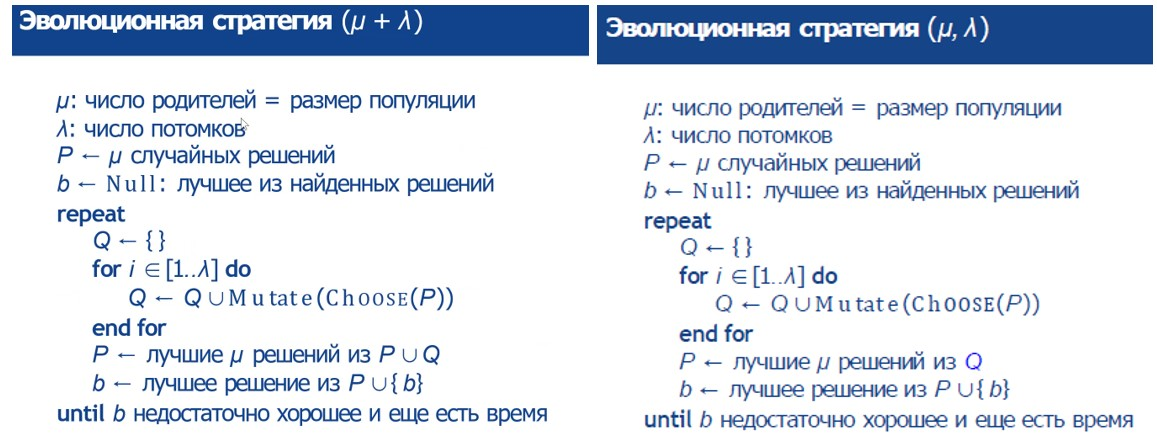
\includegraphics[width=\textwidth]{images/11bilet.jpg}   